% !TeX program = xelatex
\documentclass{article}
\usepackage{kotex}
\usepackage[a4paper,left=3cm, right=3cm, top=2cm, bottom=2cm]{geometry}
\usepackage{amsmath}
\usepackage{graphicx}
\usepackage{caption}
\usepackage{setspace}
\usepackage{xcolor}
\usepackage{titlesec}
\usepackage{amssymb}
\usepackage{tcolorbox}
\usepackage{amsthm}
\usepackage{multirow}
\usepackage{array}
\usepackage{booktabs}
\usepackage{tikz}
\usetikzlibrary{positioning,arrows.meta,calc,shapes.geometric}
\usepackage{pgfplots}
\pgfplotsset{compat=1.18}

\title{8.3 Isomorphism}
\date{}
\author{}
\setstretch{1.3}

\titleformat{name=\section, numberless}
  {\normalfont\large\bfseries\color{blue}}{}
  {0pt}{}
\geometry{a4paper, margin=1in}

\newcommand{\redheading}[1]{{\vspace{2mm}\noindent\Large\bfseries\color{red!55!black} #1\par}\vspace{2mm}}

\begin{document}
\maketitle

{\itshape\color{blue!45!black}
In this section we establish a fundamental connection between real finite-dimensional vector
spaces and the Euclidean space $R^n$. This connection is theoretically important and has
practical value: it allows vector computations in general $n$-dimensional spaces to be
performed by working with vectors in $R^n$.\par}

\vspace{2mm}

\redheading{Isomorphism}

Although many theorems in this text concern $R^n$ exclusively, every real $n$-dimensional
vector space has the same algebraic structure as $R^n$, even if its vectors are not
$n$-tuples. To make this precise, we need the following definition.

\begin{tcolorbox}[colback=teal!4, colframe=teal!65!black,
  title={\textbf{Definition 1}}, boxrule=0.5mm, arc=3mm]
A linear transformation $T : V \to W$ that is both one-to-one and onto is called an
\textbf{isomorphism}, and $W$ is said to be \textbf{isomorphic} to $V$.
\end{tcolorbox}

The following diagram illustrates an isomorphism between $P_2$ and $R^3$ via
$T(c_0+c_1x+c_2x^2) = (c_0,c_1,c_2)$; operations on one side correspond exactly to
operations on the other:

\vspace{2mm}
\begin{center}
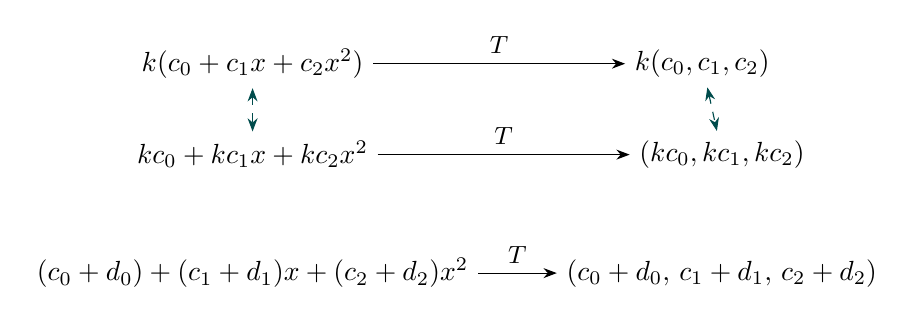
\begin{tikzpicture}[>=Stealth, node distance=0.5cm]
  \node (p1) {$k(c_0+c_1 x+c_2 x^2)$};
  \node (r1) [right=3.2cm of p1] {$k(c_0,c_1,c_2)$};
  \draw[->] (p1) -- node[above, font=\small]{$T$} (r1);
  \node (p2) [below=0.55cm of p1] {$kc_0+kc_1 x+kc_2 x^2$};
  \node (r2) [right=3.2cm of p2] {$(kc_0,kc_1,kc_2)$};
  \draw[->] (p2) -- node[above, font=\small]{$T$} (r2);
  \draw[<->, teal!60!black, dashed] (p1) -- (p2);
  \draw[<->, teal!60!black, dashed] (r1) -- (r2);
  \node (p3) [below=0.9cm of p2] {$(c_0+d_0)+(c_1+d_1)x+(c_2+d_2)x^2$};
  \node (r3) [right=1.0cm of p3] {$(c_0+d_0,\,c_1+d_1,\,c_2+d_2)$};
  \draw[->] (p3) -- node[above, font=\small]{$T$} (r3);
\end{tikzpicture}
\end{center}
\vspace{2mm}

The algebraic structure of $P_2$ is mirrored exactly in $R^3$, and vice versa via $T^{-1}$.

\begin{tcolorbox}[colback=red!4, colframe=red!60!black,
  title={\textbf{Theorem 8.3.1}}, boxrule=0.5mm, arc=3mm]
Every real $n$-dimensional vector space is isomorphic to $R^n$.
\end{tcolorbox}

\textbf{Proof.} Let $V$ be a real $n$-dimensional vector space with ordered basis
$S = \{\mathbf{v}_1, \ldots, \mathbf{v}_n\}$, and define the coordinate map $T : V \to R^n$ by
\begin{equation}
  T(\mathbf{u}) = (\mathbf{u})_S = (k_1, k_2, \ldots, k_n) \tag{2}
\end{equation}
where $\mathbf{u} = k_1\mathbf{v}_1 + \cdots + k_n\mathbf{v}_n$. Writing
$\mathbf{v} = d_1\mathbf{v}_1+\cdots+d_n\mathbf{v}_n$:
\[
  T(c\mathbf{u}) = c(k_1,\ldots,k_n) = cT(\mathbf{u}) \qquad
  T(\mathbf{u}+\mathbf{v}) = (k_1+d_1,\ldots,k_n+d_n) = T(\mathbf{u})+T(\mathbf{v})
\]
so $T$ is linear. Since distinct vectors have distinct coordinate tuples,
$T(\mathbf{u})\neq T(\mathbf{v})$ whenever $\mathbf{u}\neq\mathbf{v}$, so $T$ is one-to-one.
For any $(k_1,\ldots,k_n)\in R^n$ the vector $k_1\mathbf{v}_1+\cdots+k_n\mathbf{v}_n$
maps to it, so $T$ is onto. $\blacksquare$

\begin{tcolorbox}[colback=red!4, colframe=red!60!black,
  title={\textbf{Theorem 8.3.2}}, boxrule=0.5mm, arc=3mm]
If $S$ is an ordered basis for a vector space $V$, then the coordinate map
\[
  \mathbf{u} \;\xrightarrow{\;T\;}\; (\mathbf{u})_S
\]
is an isomorphism between $V$ and $R^n$.
\end{tcolorbox}

\textit{Remark.} Coordinate maps depend on the order of basis vectors; Theorem~8.3.2 describes
$n!$ different isomorphisms (one per ordering of the $n$ basis vectors).

\subsection*{EXAMPLE 1 | Natural Isomorphism Between $P_{n-1}$ and $R^n$}

By Theorem~8.3.2, the coordinate map with respect to the standard basis $\{1,x,\ldots,x^{n-1}\}$
defines the \textbf{natural isomorphism} between $P_{n-1}$ and $R^n$:
\[
  a_0 + a_1 x + \cdots + a_{n-1}x^{n-1} \;\xrightarrow{\;T\;}\; (a_0, a_1, \ldots, a_{n-1})
\]

\subsection*{EXAMPLE 2 | Natural Isomorphism Between $M_{22}$ and $R^4$}

The coordinate map for $M_{22}$ with respect to the standard basis gives the \textbf{natural
isomorphism} between $M_{22}$ and $R^4$:
\[
  \begin{bmatrix}a&b\\c&d\end{bmatrix} \;\xrightarrow{\;T\;}\; (a,b,c,d)
\]
More generally, the analogous map is a natural isomorphism between $M_{mn}$ and $R^{mn}$.

\subsection*{EXAMPLE 3 | Differentiation by Matrix Multiplication}
\textit{(Calculus Required)}

The differentiation $D : P_3 \to P_2$ maps
$a_0+a_1x+a_2x^2+a_3x^3 \xrightarrow{D} a_1+2a_2x+3a_3x^2$.
Under the natural isomorphisms $P_3\cong R^4$ and $P_2\cong R^3$, this corresponds to
\[
  \begin{bmatrix}0&1&0&0\\0&0&2&0\\0&0&0&3\end{bmatrix}
  \begin{bmatrix}a_0\\a_1\\a_2\\a_3\end{bmatrix}
  =
  \begin{bmatrix}a_1\\2a_2\\3a_3\end{bmatrix}
\]
For example, $\dfrac{d}{dx}(2+x+4x^2-x^3)=1+8x-3x^2$ is reproduced by
\[
  \begin{bmatrix}0&1&0&0\\0&0&2&0\\0&0&0&3\end{bmatrix}
  \begin{bmatrix}2\\1\\4\\-1\end{bmatrix}
  =
  \begin{bmatrix}1\\8\\-3\end{bmatrix}
\]
This approach is useful for numerical algorithms that compute derivatives.

\subsection*{EXAMPLE 4 | Working with Isomorphisms}

Use the natural isomorphism between $P_5$ and $R^6$ to determine whether the following
polynomials are linearly independent:
\begin{align*}
  \mathbf{p}_1 &= 1 + 2x - 3x^2 + 4x^3 + x^5\\
  \mathbf{p}_2 &= 1 + 3x - 4x^2 + 6x^3 + 5x^4 + 4x^5\\
  \mathbf{p}_3 &= 3 + 8x - 11x^2 + 16x^3 + 10x^4 + 9x^5
\end{align*}

\textbf{SOLUTION:} Form the matrix $A$ whose rows are the coordinate vectors under the
natural isomorphism:
\[
  A = \begin{bmatrix}1&2&-3&4&0&1\\1&3&-4&6&5&4\\3&8&-11&16&10&9\end{bmatrix}
\]
Row-reducing gives
\[
  R = \begin{bmatrix}1&2&-3&4&0&1\\0&1&-1&2&5&3\\0&0&0&0&0&0\end{bmatrix}
\]
$R$ has only two nonzero rows, so the row space of $A$ is two-dimensional, meaning the
rows of $A$ are linearly dependent. Therefore $\mathbf{p}_1, \mathbf{p}_2, \mathbf{p}_3$
are linearly dependent.

\vspace{2mm}

\redheading{Inner Product Space Isomorphisms}

When $V$ is a real $n$-dimensional inner product space, both $V$ and $R^n$ carry geometric
as well as algebraic structure. An isomorphism $T : V \to W$ between inner product spaces
is called an \textbf{inner product space isomorphism} if
\[
  \langle T(\mathbf{u}), T(\mathbf{v})\rangle = \langle \mathbf{u}, \mathbf{v}\rangle
  \quad\text{for all } \mathbf{u},\mathbf{v}\in V
\]
(inner product on the left is in $W$; on the right, in $V$).

To preserve geometric structure an isomorphism must preserve inner products, since length,
angle, and orthogonality all depend on the inner product. The following analog of
Theorem~8.3.2 provides an important method for obtaining inner product space isomorphisms.

\begin{tcolorbox}[colback=red!4, colframe=red!60!black,
  title={\textbf{Theorem 8.3.3}}, boxrule=0.5mm, arc=3mm]
If $S = \{\mathbf{v}_1, \mathbf{v}_2, \ldots, \mathbf{v}_n\}$ is an ordered orthonormal
basis for a real $n$-dimensional inner product space $V$, then the coordinate map
$\mathbf{u} \xrightarrow{T} (\mathbf{u})_S$ is an inner product space isomorphism between
$V$ and $R^n$ with the Euclidean inner product.
\end{tcolorbox}

\subsection*{EXAMPLE 5 | An Inner Product Space Isomorphism}

The natural isomorphism $T : P_{n-1} \to R^n$ of Example~1 maps
$a_0+a_1x+\cdots+a_{n-1}x^{n-1} \mapsto (a_0,a_1,\ldots,a_{n-1})$.
The standard basis $\{1,x,\ldots,x^{n-1}\}$ is orthonormal under the standard inner product
on $P_{n-1}$, so by Theorem~8.3.3, $T$ is an inner product space isomorphism. To verify
directly: for $\mathbf{p} = a_0+\cdots+a_{n-1}x^{n-1}$ and $\mathbf{q} = b_0+\cdots+b_{n-1}x^{n-1}$,
\[
  \langle\mathbf{p},\mathbf{q}\rangle = a_0 b_0 + a_1 b_1 + \cdots + a_{n-1}b_{n-1}
\]
which equals the Euclidean inner product of $(a_0,\ldots,a_{n-1})$ and $(b_0,\ldots,b_{n-1})$
in $R^n$. $\checkmark$

\subsection*{EXAMPLE 6 | A Notational Matter}

Let $R^n$ denote $n$-tuples in comma-delimited form and $M_n$ denote real $n\times 1$ column
matrices, with inner products $\langle\mathbf{u},\mathbf{v}\rangle = \mathbf{u}\cdot\mathbf{v}$
and $\langle\mathbf{u},\mathbf{v}\rangle = \mathbf{u}^T\mathbf{v}$ respectively. The map
\[
  T : R^n \to M_n, \qquad (v_1, v_2, \ldots, v_n) \;\longmapsto\;
  \begin{bmatrix}v_1\\v_2\\\vdots\\v_n\end{bmatrix}
\]
is an inner product space isomorphism, confirming that $R^n$ and $M_n$ are essentially the
same inner product space — a fact used throughout this text.

\vspace{3mm}
\noindent\rule{\linewidth}{0.5pt}

\section*{Exercise Set 8.3}

\noindent\textit{In Exercises 1--8, state whether the transformation is an isomorphism.
No proof required.}

\begin{enumerate}
  \item $c_0 + c_1 x \;\longmapsto\; (c_0 - c_1,\, c_1)$ from $P_1$ to $R^2$.

  \item[3.] $a + bx + cx^2 + dx^3 \;\longmapsto\; \begin{bmatrix}a&b\\c&d\end{bmatrix}$
        from $P_3$ to $M_{22}$.

  \item[5.] $(a,b,c,d) \;\longmapsto\; a + bx + cx^2 + (d+1)x^3$ from $R^4$ to $P_3$.

  \item[6.] $A \;\longmapsto\; A^T$ from $M_{nn}$ to $M_{nn}$.

  \item[7.] $c_1\sin x + c_2\cos x \;\longmapsto\; (c_1, c_2)$ from the subspace of
        $C(-\infty,\infty)$ spanned by $\{\sin x, \cos x\}$ to $R^2$.

\end{enumerate}

\begin{enumerate}
  \item[9.] \textbf{a.} Find an isomorphism between the vector space of all $3\times 3$
        symmetric matrices and $R^6$.\\
        \textbf{b.} Find two different isomorphisms between the vector space of all
        $2\times 2$ matrices and $R^4$.

  \item[10.] \textbf{a.} Find an isomorphism between the vector space of all polynomials
        in $P_3$ satisfying $p(0) = 0$ and $R^3$.

\end{enumerate}

\noindent\textit{In Exercises 11--12, use Theorem 8.2.2 to determine whether
$T_A : R^3 \to R^3$ is an isomorphism.}

\begin{enumerate}
  \item[11.] $A = \begin{bmatrix}0&1&-1\\1&0&2\\-1&1&0\end{bmatrix}$

\end{enumerate}

\noindent\textit{In Exercises 13--14, find the dimension $n$ of the solution space $W$
of $A\mathbf{x} = \mathbf{0}$, then construct an isomorphism between $W$ and $R^n$.}

\begin{enumerate}
  \item[13.] $A = \begin{bmatrix}1&1&1&1\\2&2&2&2\\3&3&3&3\end{bmatrix}$

\end{enumerate}

\noindent\textit{In Exercises 15--16, determine whether the transformation is an isomorphism
from $M_{22}$ to $R^4$.}

\begin{enumerate}
  \item[15.] $\begin{bmatrix}a&b\\c&d\end{bmatrix} \;\longmapsto\;
        \begin{pmatrix}a \\ a+b \\ a+b+c \\ a+b+c+d\end{pmatrix}$

\end{enumerate}

\begin{enumerate}
  \item[17.] Is $R^2$ isomorphic to the $xy$-plane in $R^3$? Justify your answer.

  \item[19.] Let $T : P_2 \to M_{22}$ be defined by
        \[
          T(p(x)) = \begin{bmatrix}p(0) & p(1)\\p(1) & p(0)\end{bmatrix}
        \]
        Is $T$ an isomorphism? Justify your answer.

\end{enumerate}

\noindent\textit{Working with Proofs}

\begin{enumerate}
  \item[22.] Prove: if $T : V \to W$ is an isomorphism, then $T^{-1} : W \to V$ is also
        an isomorphism.

  \item[25.] Prove that an inner product space isomorphism preserves angles and
        distances: the angle between $T(\mathbf{u})$ and $T(\mathbf{v})$ in $W$ equals
        the angle between $\mathbf{u}$ and $\mathbf{v}$ in $V$, and
        $\|T(\mathbf{u}) - T(\mathbf{v})\|_W = \|\mathbf{u} - \mathbf{v}\|_V$.

\end{enumerate}

\end{document}
